\chapter{背侧前额叶皮层:基于最近事件生成目标}
背侧PF皮层有助于根据顺序、时间和空间环境生成目标,它的连接解释了为什么只有它才能做到这一点。背侧PF皮层,包括中外侧PF皮层(46区),通过与后顶叶皮层、前运动皮层和PF皮层的其他部分连接来发挥作用。顶叶连接提供了许多用于生成目标的空间和时间背景。与运动前区域的联系导致这些目标的实现,通常是通过手的运动。与眶侧PF皮层的连接使背侧PF皮层能够根据单个事件预测目标选择的具体结果。背侧PF皮层位于背侧视觉流的末端,因此它可以规划目标序列,它可以具体或抽象地指定这些目标。在产生目标后,背侧PF皮层可以前瞻性地编码它们,直到行动的时候到来。鉴于背侧PF皮层在类人猿灵长类动物中进化(第2章),我们认为它在使用最近视觉事件的顺序、时间和位置来指导觅食选择和生成效率优化的目标序列方面具有优势。

\section{介绍}
第二章解释了灵长类动物的PF皮层在类人猿中随着新区域的出现而扩展。第三章涉及了其中的一些,例如极性PF皮层(10区),但在本章和下一章,它们是主要主题。由于类人猿依赖于白天漫长的觅食旅行,它们需要消耗大量的能量,并面临着很高的捕食风险。这种生活方式非常重视正确的觅食选择。在影响这种选择的因素中,视觉事件的位置、时间和顺序是突出的,因为类人猿利用了它们在中央凹和色彩视觉方面的进步。正如第二章所解释的,这些进步包括中央凹提供的精致的视觉敏锐度和三色视觉提供的增强的辨别能力。

这一章解释了觅食的选择部分取决于当前的环境,这是由选择时可用的刺激以及最近视觉事件的记忆所指定的。为了理解我们的意思,考虑一个简单的实验室任务:延迟匹配样本。猴子把一个刺激看作一个样本,然后看到一个或多个刺激需要选择。这种选择不仅取决于选择时的刺激,还取决于基于样本刺激的记忆。这两个因素共同构成了当前选择目标的背景。

由于记忆对当前情境起作用,这类实验的被试面临一个问题:最近发生了几件事,并选择了几个目标。本章的大部分内容探讨了背侧PF皮层如何帮助类人猿灵长类动物解决这个问题。许多文献都依赖于一个任务和一个区域:延迟反应任务,它依赖于中外侧PF皮层(46区)。因此,我们将讨论的重点放在第一章和第五章也提到的这个任务上。我们认为,因为受试者在这个任务中经历了一系列的视觉事件,并实现了一系列的目标,他们需要挑选出决定当前目标的事件。然后,我们回顾一系列其他任务,这些任务也要求主体在当前环境的基础上生成目标。
\section{区域}
在猕猴中,中外侧PF皮层位于主枕沟的吻侧三分之二(图6.1)。然而,它也延伸到这个沟的背侧和腹侧的凸面皮层。中外侧PF皮层(46区)有很多名字,有些很明确,有些则不太明确。
\begin{figure}
	\centering
	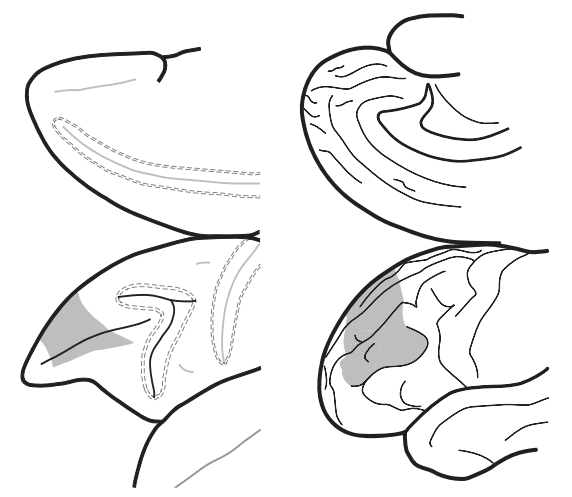
\includegraphics[width=0.7\linewidth]{image_pfc/Fig_6_1}
	\caption{猕猴(左)和人类(右)的背侧PF皮层。格式如图1.2所示}
	\label{fig:fig}
\end{figure}

Walker(1940)将沿主沟整个长度的皮层称为46区,但最近Petrides和Pandya(1999)将9/46区区分为该沟的尾端周围(见图1.2)。为了避免对46这个术语的不同用法的混淆,我们称沃克46区吻侧三分之二为中外侧PF皮层,尾侧三分之一为后外侧PF皮层。在人类中,这些分区位于额上回和额下沟之间。

尽管出现了这些新术语,但混淆的空间仍然很大。术语背侧前额叶皮层最初是指猴子的整个侧前额叶皮层(Pribram et al. 1952),但后来仅指主沟内和背侧的皮层(Mishkin et al. 1969)。在影像学文献中,指PF背外侧皮层已变得很常见,但该术语的使用通常非常松散,很少注意解剖标志。因此,我们在本书中避免使用这个术语。表1.2给出了我们所采用的术语。我们将PF背侧皮层包括主沟两岸的皮层和其背侧的凸面皮层(区域9),但不包括区域9的内侧部分。当然,这些划分并不是最终的结果,但它们在一定程度上反映了联系。
\section{连接}
图6.2展示了PF皮层背侧的一些皮质连接。正如第一章所解释的,这些连接构成了解剖指纹。
\par
1.中外侧PF皮层(46区)与后顶叶皮层,特别是尾顶叶区有很强的联系(Petrides \& Pandya 1984,1999,2009)。正如前一章所提到的,后顶叶皮层的许多神经元编码视觉空间信息。然而,顶叶细胞也编码时间间隔(Leon \& Shadlen 2003),当人类受试者对近期事件做出判断时,左侧顶叶内沟会出现激活(Dudukovic \& Wagner 2007)。
\par
2.中外侧PF皮层连同外侧9区,与位于颞上沟上岸的多模态区TPO区(也称为颞上多感觉区STP)相连(Seltzer et al. 1996;Petrides \& Pandya1999)。该区域的细胞对体感、听觉和视觉刺激有反应(Bruce et al. 1981)。
\par
3.中外侧PF皮层也接受来自周围皮层的输入(Petrides \& Pandya 1999),其功能是识别物体(Murray et al. 2007)。这种联系表明,中外侧前额叶皮层接收到有关物体的直接输入,而不仅仅是腹侧前额叶皮层的间接输入(第7章和第8章)。
\par
4.中外侧前额叶皮层接收来自次级体感觉区(S2) (Petrides \& Pandya 2002b)和下颞叶皮层吻侧PFG区(Rozzi etal . 2006)的输入。这些区域的细胞对体感刺激有反应(Hyvarinen 1981),中外侧PF皮层的细胞也是如此(Tanila et al. 1993)。这一特征将中外侧PF皮层与尾侧和后外侧PF皮层区分开来,后者的细胞主要具有视觉和注意力特性(第5章)。
\par
5.中外侧PF皮层连接背侧和腹侧前运动皮层(Wang et al. 2002),以及前辅助运动区(preSMA) (Wang et al. 2005)和位于扣带沟的扣带吻侧运动区(CMAr) (Dum \& Strick 1993)。这些投影主要涉及代表手和手臂的运动前区域,而不是脚和腿。前肢表征的专门化表现在背侧前前皮层的吻侧部分(Tachibana et al. 2004)、腹侧前运动皮层(He et al. 1993)、preSMA (Luppino et al. 1991)和CMAr (He et al. 1995)。因此,相对于运动的运动,中外侧PF皮层在伸手、操作和进食运动中具有优先的作用(第2章)。
\par
6.中外侧PF皮层与前扣带皮层有很强的联系(Petrides \& Pandya 1999)。第3章解释了前扣带皮层在动作的评估和基于这些评估的动作之间的切换中发挥作用(Walton et al. 2007)。
\par
7.中外侧PF皮层与脾后皮层相连(Morris et al. 1999)。反过来,从脾后皮层投射到海马旁回和下丘前(Kobayashi \& Amaral 2007)。我们认为,这些联系可能在有关事件的记忆检索中发挥作用,而这种检索依赖于时间或空间上下文(Vann et al. 2009)。
\par
8.区域9的横向部分的连接受到的关注相对较少,部分原因是很少有功能数据引起人们的兴趣。这部分背侧PF皮层与背侧运动前皮层的吻侧部分(Petrides \& Pandya 1999)和CMAr (Morecraft \& van Hoesen 1993)有联系。就像第9区域的内侧部分一样,它也与上颞皮质有联系,这可能传达听觉信息(Petrides \& Pandya 1984;Saleem et al. 2008)。最后,第9区外侧部分与后顶叶皮层下部(PG区)(Cavada \& Goldman-Rakic 1989)和脾后皮层(Kobayashi \& Amaral 2003)相连。
\begin{figure}
	\centering
	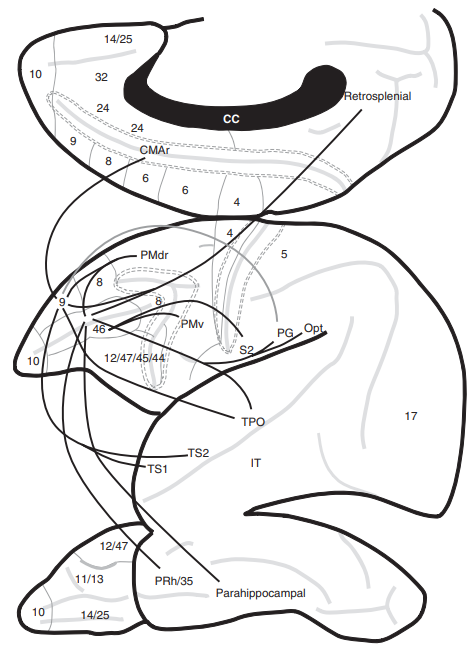
\includegraphics[width=0.7\linewidth]{image_pfc/Fig_6_2}
	\caption{PF皮层背侧的选定连接。图1.4和1.5给出了沟和区域的名称。一些轴突与背侧PF皮层有直接连接的区域被认为是相互的,除非另有说明}
	\label{fig:fig}
\end{figure}

\subsection{总结}
中外侧PF皮层与后顶叶皮层、前运动皮层有很强的联系,并间接与海马系统有联系。它也与PF皮层的其他部分相互连接,如眶PF皮层。其他皮质区域没有这种连接模式。因此,它很好地整合了由眶前PF皮层、背侧视觉流和海马体处理的信息,并向运动前皮层提供信息。

\section{指纹}

\subsection{损伤和激活}

\subsection{损伤和活动}

\subsection{活动和激活}




\subsection{结论}


